\chapter{High-Level Design}
\label{chap:high-level-design}

\section{Introduction}
The High-Level Design (HLD) defines the structural blueprint of the Nexus PM platform. It establishes the relationship between business-level functional requirements and the physical infrastructure, logical containers, and system components that execute them. The purpose of this chapter is to provide system architects, developers, and operations engineers with a clear understanding of the overall topology, component boundaries, data pathways, and integration schemas that define the platform.

By articulating the design from system context down to component interactions, this design ensures that the implementation satisfies operational goals for performance, security, and scalability.

\section{Architectural Goals}
The design of Nexus PM is driven by eight core engineering and operational objectives:
\begin{itemize}
    \item \textbf{Horizontal Scalability:} The application tier must remain stateless to support horizontal autoscaling behind load balancers, adapting compute resources to active user traffic.
    \item \textbf{Codebase Maintainability:} By separating database queries, business rules, and API routing, the system remains easy to update, test, and refactor.
    \item \textbf{Cloud-Native Extensibility:} Built around managed APIs and serverless resources (e.g., Supabase, Upstash, Cloudflare R2), the system minimizes database administration overhead while maintaining access control standards.
    \item \textbf{System Modularity:} Backend modules must be partitioned into clear packages (Authentication, Projects, Tasks, Storage, AI) to simplify eventual microservices refactoring.
    \item \textbf{Rigid Security Posture:} Transport encryption, secure cookie containment, stateless session authentication, and row-level access permissions are enforced across all integration points.
    \item \textbf{Sub-Second Performance:} The platform must achieve sub-second response times by leveraging client-side state caching and server-side in-memory read caching.
    \item \textbf{Graceful Fault Tolerance:} External service dependencies (e.g., AI gateways, email APIs) are isolated via asynchronous queues and exception boundaries, preventing external outages from impacting core task tracking functions.
    \item \textbf{Developer Experience (DX):} The architecture must support local development environments using Docker container scaffolding and automatically generated OpenAPI documentation.
\end{itemize}

\section{Architectural Principles}
The platform incorporates several software design principles to ensure reliability and maintainability:
\begin{itemize}
    \item \textbf{Decoupled Layering:} Decouples the presentation client from the backend business rules engine. Communication occurs exclusively over standard HTTPS endpoints.
    \item \textbf{Separation of Concerns (SoC):} Logical layers (Data Access, Service Logic, API Controllers) have distinct boundaries, preventing database operations from leaking into router interfaces.
    \item \textbf{Stateless Execution:} The API gateway preserves no session state on local disk or memory. All user sessions are validated statelessly using cryptographically signed JSON Web Tokens (JWT).
    \item \textbf{Dependency Injection (DI):} Database sessions, security handlers, and external API clients are dynamically injected at runtime, simplifying unit testing and mocking.
    \item \textbf{Repository Design Pattern:} All SQL executions are encapsulated within dedicated Repository classes, isolating the SQLAlchemy ORM details from service-level workflows.
    \item \textbf{Single Responsibility Principle (SRP):} Each controller, service helper, and data repository is responsible for a single area of system functionality.
    \item \textbf{Asynchronous Task Processing:} Long-running computational processes, email dispatches, and LLM calls are handled asynchronously, preventing thread starvation in the primary web gateway.
\end{itemize}

\pagebreak
\section{System Context}
The system context defines the operational boundaries of Nexus PM, outlining how users and external services interact with the platform core. Figure~\ref{fig:system_architecture} illustrates these boundaries and integration points.

\begin{figure}[h!]
    \centering
    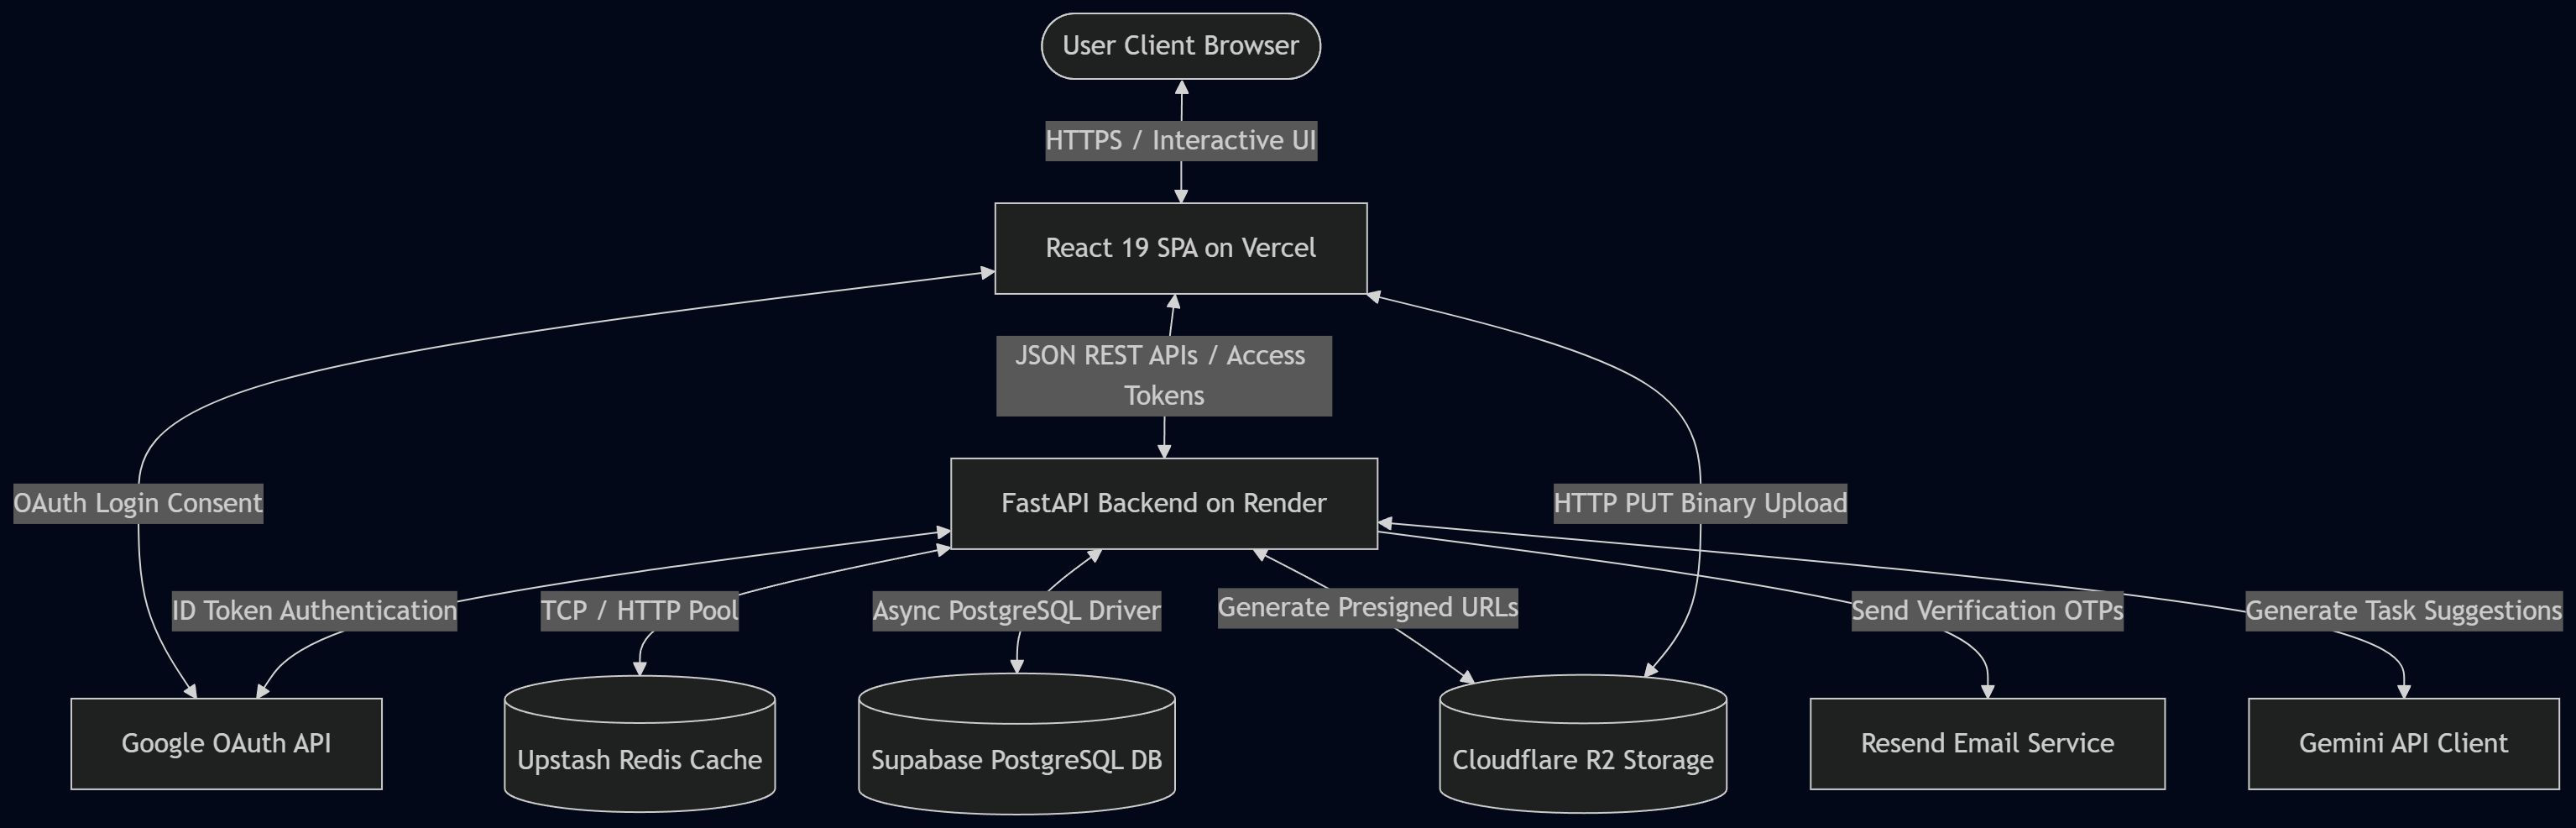
\includegraphics[width=\textwidth]{figures/system-architecture.png}
    \caption{Nexus PM System Context and Integration Topology}
    \label{fig:system_architecture}
\end{figure}

The system boundary encompasses the frontend application and the backend API service. Users access the system via modern web browsers using HTTPS. External interactions include:
\begin{itemize}
    \item \textbf{Google OAuth Gateway} for secure federated authentication.
    \item \textbf{Supabase Managed Database} for transactional storage.
    \item \textbf{Upstash Redis} for rate limiting, session cache, and system state storage.
    \item \textbf{Cloudflare R2} for S3-compatible, zero-egress asset storage.
    \item \textbf{Google Gemini AI} for structured task breakdown and summarization.
    \item \textbf{Resend API} for automated transactional email delivery.
\end{itemize}

\section{Container Architecture}
The logical containers of Nexus PM are split across client, server, and storage clusters, as detailed in the deployment architecture shown in Figure~\ref{fig:deployment_architecture}.

\begin{figure}[h!]
    \centering
    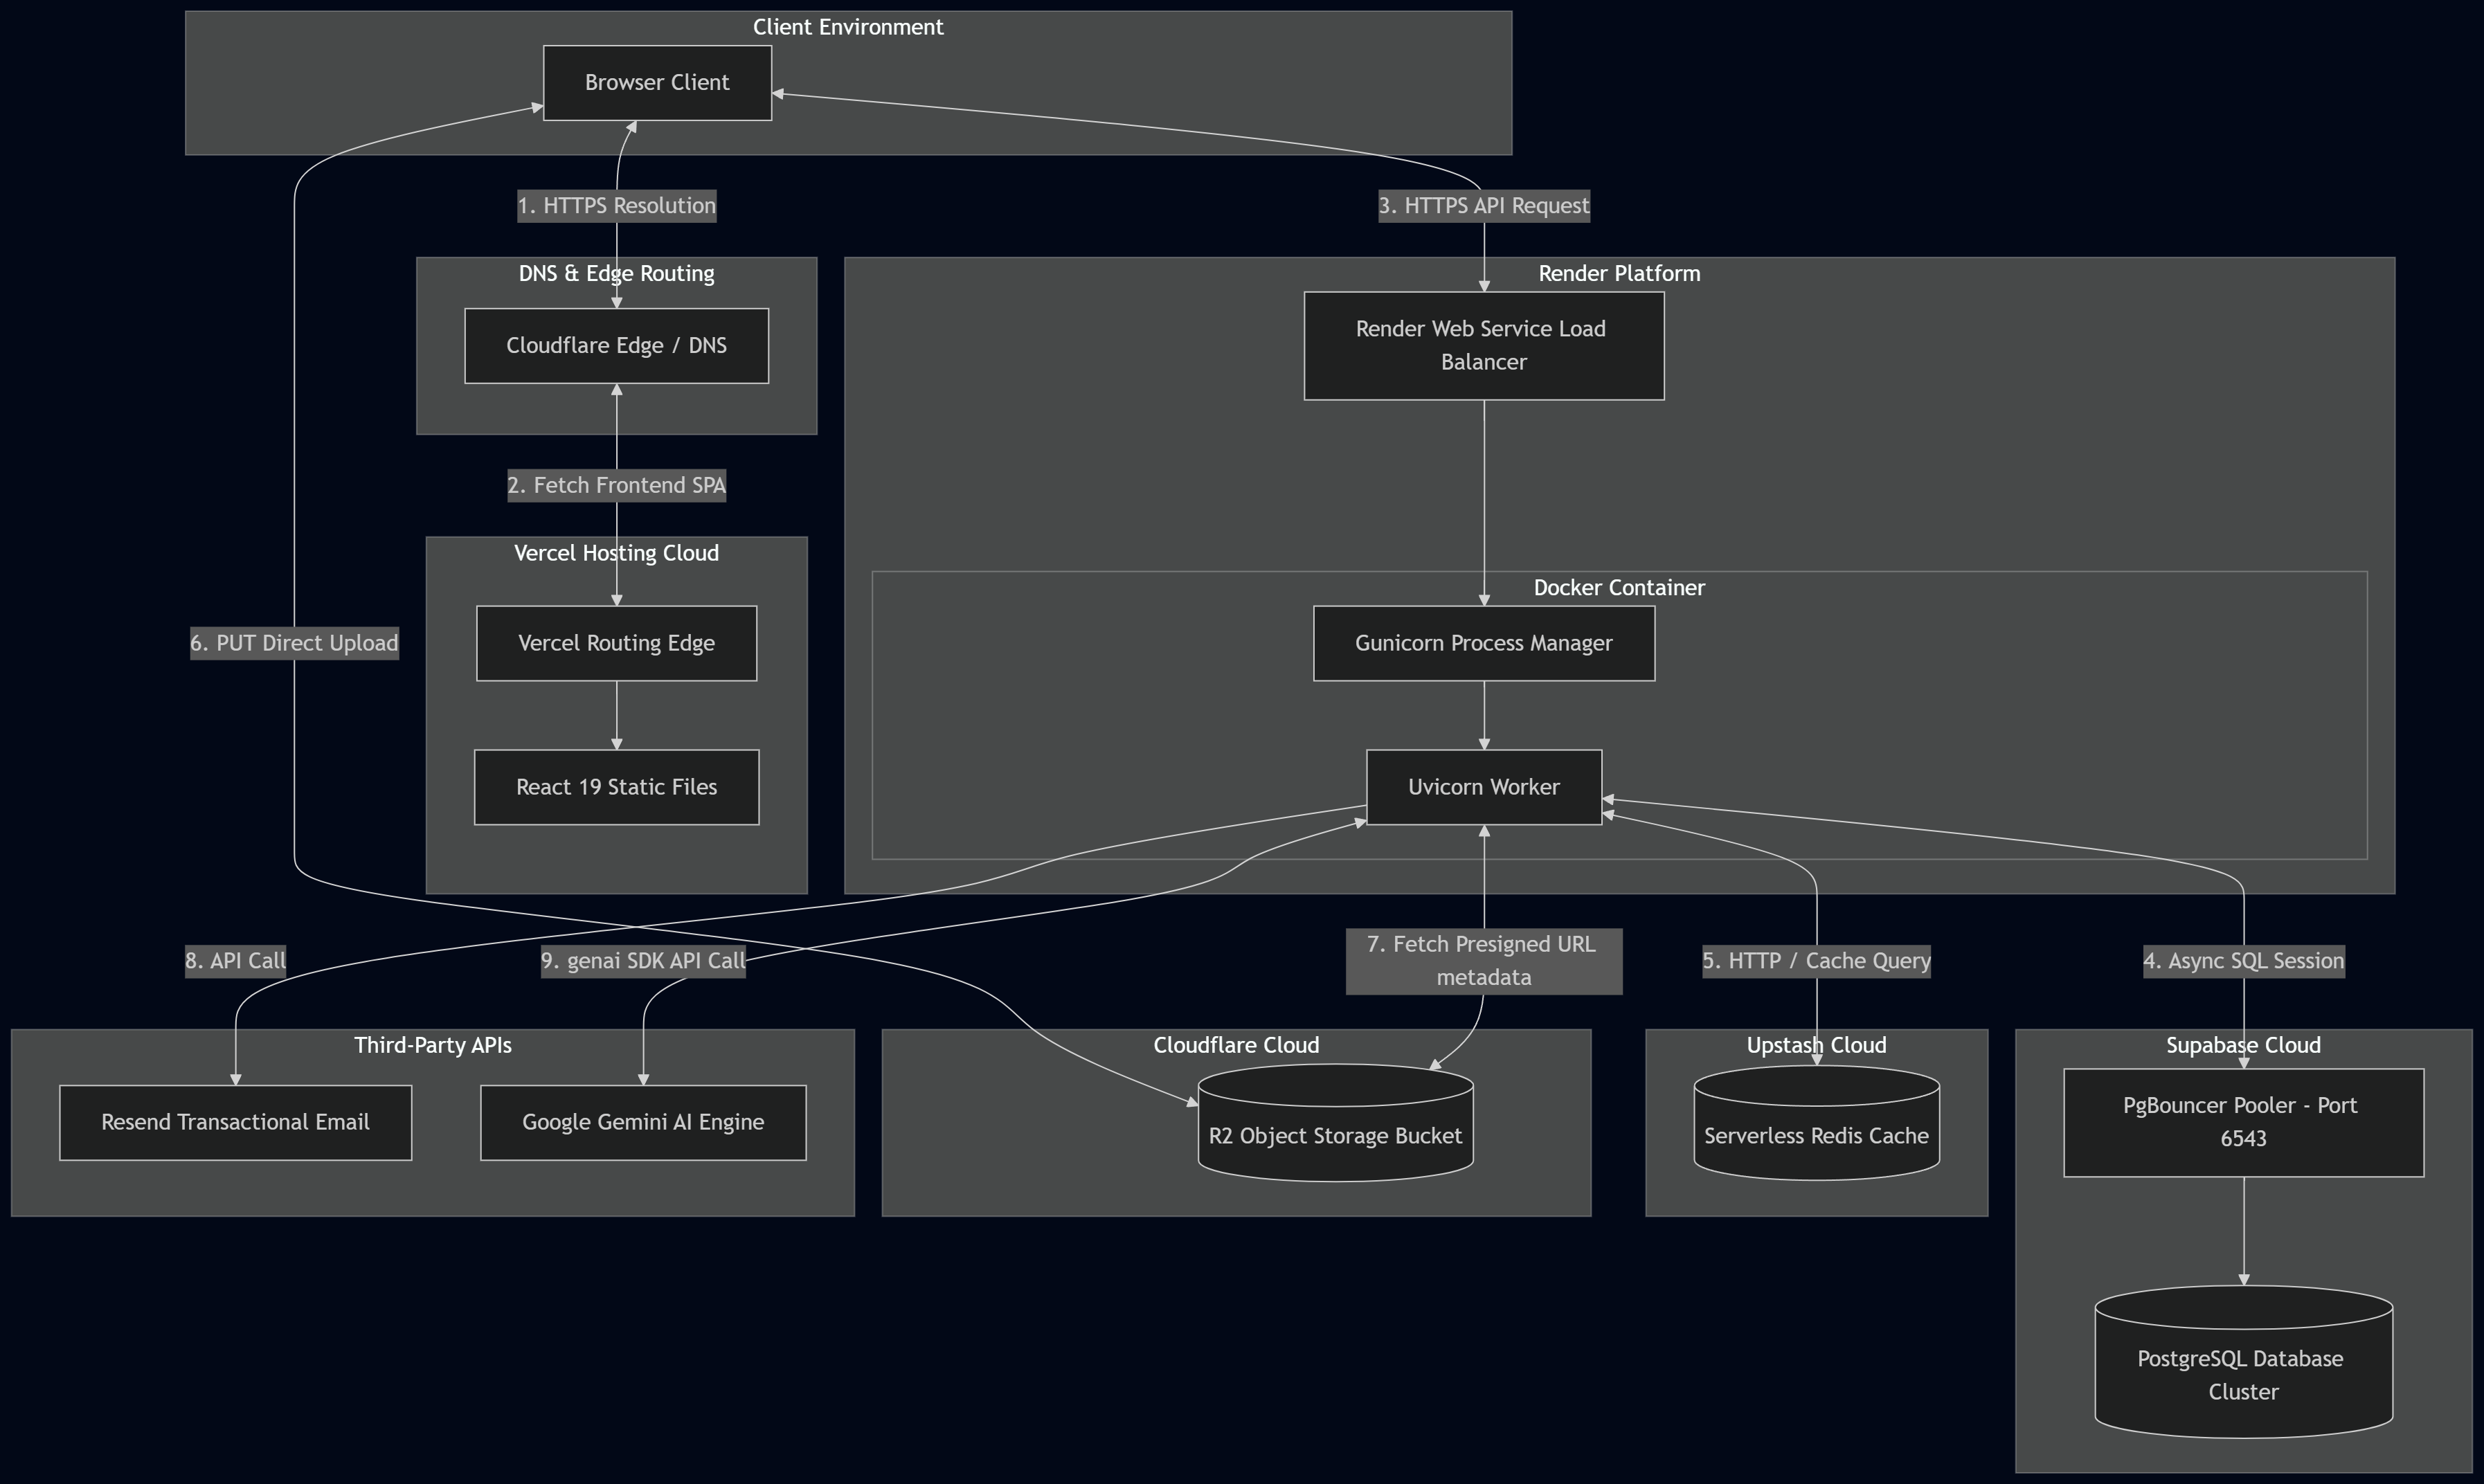
\includegraphics[width=\textwidth]{figures/deployment-architecture.png}
    \caption{Nexus PM Production Container Topologies and Networking}
    \label{fig:deployment_architecture}
\end{figure}

\begin{itemize}
    \item \textbf{Client Container (Vercel CDN):} Serves the compiled React 19 single-page application. Static assets are cached at edge nodes globally, offloading static file serving from the backend.
    \item \textbf{Backend Container (Render Web Service):} Executes the stateless FastAPI python app inside a multi-stage Docker environment. It manages route handling, input validation, service coordination, and access rule checks.
    \item \textbf{Database Container (Supabase Managed Service):} Hosts the PostgreSQL engine, enforcing table constraints, primary key relations, index tracking, and transactional safety.
    \item \textbf{In-Memory Cache (Upstash Redis):} Serves as a low-latency key-value store, handling active user session metadata, API rate-limiting buckets, and temporary database read-caches.
    \item \textbf{Object Store Container (Cloudflare R2):} Manages raw binary files (images, PDF documents, attachments) using access-controlled bucket permissions, bypassing database storage limits.
    \item \textbf{AI Processing Container (Google API Gateway):} Processes prompt variables, runs generative model parameters, and outputs structured JSON data back to the backend.
\end{itemize}

\section{Component Architecture}
The internal structure of the backend application consists of decoupled components communicating through defined interfaces:
\begin{itemize}
    \item \textbf{Authentication Component:} Manages secure identity assertion. It verifies JWT signatures, coordinates refresh token rotations, and exchanges Google OAuth tokens for authenticated sessions.
    \item \textbf{Projects Component:} Handles workspaces, projects, and workspace memberships. It verifies project state, updates membership metadata, and enforces tenant isolation.
    \item \textbf{Tasks Component:} Governs task entities, Kanban lanes, attachments, comments, and task assignments. It tracks state modifications and triggers notification dispatch jobs.
    \item \textbf{Storage Component:} Validates attachment parameters (file extensions, maximum sizes) and generates short-lived pre-signed R2 upload URLs.
    \item \textbf{Notification Component:} Formats invite emails and status update alerts, forwarding structured payloads to the Resend API.
    \item \textbf{Analytics Component:} Calculates task velocities, workload balances, and overall completion percentages across active workspaces using optimized database aggregation queries.
    \item \textbf{AI Orchestration Component:} Builds context payloads, validates structured LLM formatting requirements, and manages background prompt execution queues.
    \item \textbf{Database Access Layer (SQLAlchemy ORM):} Provides mapping between database schemas and Python objects, executing transactions using connection pooling pools.
\end{itemize}

\section{Request Lifecycle}
To illustrate the data paths across these logical components, the execution path of a complex transactional request (e.g., creating a task with automated AI task decomposition) is detailed below:
\begin{enumerate}
    \item \textbf{Client Dispatch:} The user submits a task creation request on the React client. The client client packages the input details and issues a POST request, appending the session JWT in the secure request cookie.
    \item \textbf{Gateway Route Handling:} The FastAPI backend receives the request. The gateway executes validation checks, checking the JWT signature and verifying that the user has the required workspace role.
    \item \textbf{Rate Limiting Check:} The backend calls Upstash Redis to verify that the user ID has not exceeded rate-limiting thresholds.
    \item \textbf{Relational Database Transaction:} The service layer maps the request data to a SQLAlchemy ORM model and opens a PostgreSQL transaction. The task is created, database constraints are validated, and the transaction is committed.
    \item \textbf{Asynchronous Task Triggering:} With the primary task saved, the service layer dispatches an asynchronous background task to call the AI orchestration component for task decomposition.
    \item \textbf{HTTP Response Resolution:} The backend immediately returns the created task data to the client, keeping the user interface active while the background processes run.
    \item \textbf{AI Generation \& Database Commit:} The background AI worker compiles the task context, formats the prompt template, and sends a secure request to Google Gemini 2.5 Flash. The model returns a structured JSON payload of sub-tasks. The worker validates the output and saves the sub-tasks to Supabase.
    \item \textbf{Notification Dispatch:} Upon database commit, the worker triggers the notification service, which formats an assignment email and dispatches it via Resend.
    \item \textbf{Client State Refresh:} The React client, listening for changes or polling the endpoint via React Query, receives the updated sub-task data, refreshing the UI view.
\end{enumerate}

\section{Technology Stack Overview}
Table~\ref{tab:hld_tech_stack} details the technologies selected for Nexus PM along with their core architectural responsibilities.

\begin{table}[h!]
\centering
\small
\renewcommand{\arraystretch}{1.5}
\begin{tabularx}{\textwidth}{l l X}
    \toprule[1.5pt]
    \rowcolor{primary!5}
    \textbf{\color{primary}Technology} & \textbf{\color{primary}Layer} & \textbf{\color{primary}Architectural Role} \\
    \midrule
    React 19 & Client & Single-page application rendering, virtual DOM state synchronization. \\
    TypeScript & Client & Type checking at compile-time to reduce runtime execution errors. \\
    Redux Toolkit & Client & Centralized client state cache for application layout rules. \\
    React Query & Client & Data synchronization, caching, and automatic refetch policies. \\
    Tailwind CSS & Client & Declarative, atomic UI layout styling. \\
    FastAPI & Backend & High-throughput REST API gateway with native asynchronous support. \\
    SQLAlchemy & Backend & Object-relational mapping, connection pooling, and schema isolation. \\
    Supabase (PostgreSQL) & Storage & Persistent relational database, transaction safety, and database indexes. \\
    Upstash Redis & Cache & Serverless cache registry, session cache, and rate-limiter tracker. \\
    Cloudflare R2 & Storage & S3-compatible secure object storage for project attachments. \\
    Resend API & Gateway & API-driven transactional email dispatching. \\
    Google Gemini 2.5 Flash & AI & Large Language Model for task decomposition and project updates. \\
    Docker & Operations & Multi-stage container packaging for runtime environment parity. \\
    \bottomrule[1.5pt]
\end{tabularx}
\caption{Nexus PM Technology Stack Architecture Roles}
\label{tab:hld_tech_stack}
\end{table}

\section{External Service Integration}
Integrating third-party managed services allows the platform to maintain a low operational footprint:
\begin{itemize}
    \item \textbf{Supabase:} Provides a managed PostgreSQL instance, eliminating database hosting, provisioning, and configuration overhead.
    \item \textbf{Cloudflare R2:} Handles raw binary uploads, removing the storage and egress bandwidth costs associated with traditional cloud file storage providers.
    \item \textbf{Upstash Redis:} Delivers a serverless cache layer that dynamically scales based on request volume, avoiding the need to run and maintain dedicated Redis instances.
    \item \textbf{Resend:} Provides high email deliverability through a clean API wrapper, avoiding complex SMTP configurations.
    \item \textbf{Google OAuth:} Delegates identity verification to Google's authentication infrastructure, minimizing the risks associated with local credential storage.
    \item \textbf{Google Gemini API Gateway:} Integrates advanced generative reasoning capabilities, providing structured JSON outputs based on raw prompt parameters.
\end{itemize}

\pagebreak
\section{Deployment Overview}
The production deployment configuration relies on distributed cloud providers, coordinated as shown in Figure~\ref{fig:deployment_architecture}:
\begin{itemize}
    \item \textbf{Client Hosting (Vercel):} React static resources are built and distributed across Vercel's global CDN locations, ensuring low latency for initial page loads.
    \item \textbf{Web Service Compute (Render):} The backend Docker container is hosted on Render, which manages health-check routing, automated deployments on git push, and automatic scaling groups.
    \item \textbf{Managed Database (Supabase):} Database instances run in isolated cloud environments, connecting securely over TLS using PgBouncer connection pooling.
    \item \textbf{Serverless Cache (Upstash):} Managed Redis instances run in close physical proximity to Render's compute nodes to minimize cache access latencies.
\end{itemize}

\section{Design Decisions}
Several key architectural trade-offs were made during the design of Nexus PM:
\begin{itemize}
    \item \textbf{Supabase vs. Self-Managed PostgreSQL:} Using Supabase eliminated database administration overhead (backups, security patches, indexing maintenance) on the free tier, allowing the team to focus on core project management features.
    \item \textbf{Cloudflare R2 vs. AWS S3:} Cloudflare R2 was selected over AWS S3 due to its zero-egress fee pricing model. For a zero-budget project, this prevents unexpected bandwidth costs from file uploads and downloads.
    \item \textbf{Resend vs. AWS SES:} Resend was chosen for its developer-friendly setup, native JSON template integration, and fast domain validation, avoiding the complex IAM setup required by AWS SES.
    \item \textbf{Render Free Tier Container Hosting:} Packaging the application in Docker allows it to run on Render's free tier, maintaining a clear migration path to platforms like AWS ECS or Kubernetes if resource limits are exceeded.
    \item \textbf{Google Gemini 2.5 Flash vs. Alternative LLMs:} Gemini 2.5 Flash was chosen for its low request latencies, structured JSON schema output support, and generous free-tier API quotas.
\end{itemize}

\section{Strengths}
The High-Level Design of Nexus PM delivers several structural advantages:
\begin{itemize}
    \item \textbf{Complete Client-Backend Separation:} Allows independent scaling, testing, and deployment of the frontend application and backend API service.
    \item \textbf{Optimized Database Connection Management:} PgBouncer connection pooling prevents database connection exhaustion within free-tier limits.
    \item \textbf{Non-Blocking Asynchronous Operations:} Offloading heavy AI and notification tasks to background threads preserves fast API response times.
    \item \textbf{Cost-Efficient Operations:} Leveraging serverless, zero-egress cloud resources allows the platform to support scale at a fraction of the cost of traditional monolithic deployments.
\end{itemize}

\section{Chapter Summary}
This chapter detailed the High-Level Design of the Nexus PM platform, defining the system boundaries, container architecture, logical components, request lifecycles, and deployment topologies. By leveraging managed cloud components and separating client interfaces from the core business logic, the platform achieves high performance and low operational costs. The next chapter will build on these blueprints, detailing the database schemas, API routes, and code-level models in the Low-Level Design (LLD).
